\documentclass[preprint]{elsarticle}
\usepackage[utf8]{inputenc}
\usepackage{amsmath}
\usepackage{amsfonts}
%\usepackage{tikz}
%\usetikzlibrary{shapes.misc,shadows}
%\usetikzlibrary{positioning} 
\usepackage{amsthm}
\usepackage{array}
\usepackage{parskip}
\usepackage{float}
\usepackage{paralist}
\usepackage{listings}
\usepackage{color}
\usepackage{caption}
\usepackage{hyperref}
\usepackage{multirow}
\usepackage{caption}
\usepackage{subcaption}
\usepackage{tikz}
\usetikzlibrary{shapes.misc,shadows}
\usetikzlibrary{quotes,positioning,arrows,decorations.markings}
\usetikzlibrary{positioning} 
\usepackage[cache=false,section]{minted}
\usepackage[a4paper, total={6in, 8in}]{geometry}
\usepackage[tworuled,algosection,figure,linesnumbered]{algorithm2e}
\usepackage{glossaries}
\usemintedstyle{default}
\newminted{haskell}{frame=lines,framerule=2pt}
\newminted{R}{frame=lines,framerule=2pt}
\graphicspath{{./images/}}

\bibliographystyle{abbrvnat}

\newacronym{dp}{DPP}{Dynamic Pipeline Paradigm}
\newacronym{dph}{DP-Haskell}{$DP_{WCC}$ in Haskell}
\newacronym{bfs}{BFS}{Breadth-First Search}
\newacronym{dfs}{DFS}{Depth-First Search}
\newacronym{wcc}{WCC}{Weak Connected Components}
\newacronym{hs}{Haskell}{Haskell Programming Language}
\newacronym{fp}{FP}{Functional Programming}
\newacronym{stm}{STM}{Software Transactional Memory}
\newacronym{rl}{R}{R Language}
\newacronym{os}{OS}{Operative System}
\newacronym{dm}{Dm}{Diefficency Metrics}
\newacronym{tfft}{TFFT}{Time for the first tuple}
\newacronym{et}{ET}{Execution Time}
\newacronym{comp}{Comp}{Completeness}
\newacronym{tt}{T}{Throughput}
\newacronym{dt}{dief$@$t}{Diefficiency first $t$ time units}
\newacronym{snap}{SNAP}{Stanford Network Data Set Collection}
\newacronym{ghc}{GHC}{Glasgow Haskell Compiler}

\glsdisablehyper

\newcommand{\dpwcc}{\mathsf{DP_{WCC}}}
\newcommand{\iwcc}{\mathsf{I}}
\newcommand{\owcc}{\mathsf{O}}
\newcommand{\fwcc}{\mathsf{F}} 
\newcommand{\gwcc}{\mathsf{G}}
\newcommand{\ice}{\mathsf{IC_E}}
\newcommand{\csofv}{\mathsf{IC_{set(V)}}}
\newcommand{\sgen}{\mathsf{S_G}}
\newcommand{\sfilter}{\mathsf{S_F}}
\newcommand{\sinp}{\mathsf{S_I}}
\newcommand{\sout}{\mathsf{S_O}}
\newcommand{\istream}{\mathsf{D}}
\newcommand{\wccout}{\mathsf{R}}
\newcommand{\fmem}{\mathsf{M_F}}
\newcommand{\eof}{\mathsf{eof}}
\newcommand{\Act}{\mathsf{actor_1}}
\newcommand{\Actt}{\mathsf{actor_2}}
\newcommand*{\listingautorefname}{listing}



\newtheorem{thm}{Theorem}
\newtheorem{lem}[thm]{Lemma}
\newdefinition{prob}{Problem}
\newdefinition{defin}{Definition}
\newdefinition{rmk}{Remark}
\newproof{pf}{Proof}
\newproof{pot}{Proof of Theorem \autoref{thm2}}

%\title{Towards a Haskell Abstraction of Dynamic Pipeline %Paradigm\tnoteref{t1}}

\title{Towards a Dynamic Pipeline Framework implemented in (parallel) Haskell\tnoteref{t1}}

\tnotetext[t1]{This work has been partially supported by  MINECO and FEDER funds under grant TIN2017-86727-C2-1-R.}
%
\author[1]{Juan Pablo Royo Sales}
\ead{juan.pablo.royo@estudiantat.upc.edu}

\author[1]{Edelmira Pasarella}
\ead{edelmira@cs.upc.edu}

\author[1]{Cristina Zoltan}
\ead{zoltan@cs.upc.edu}

\author[2]{Maria-Esther Vidal}
\ead{maria.vidal@tib.eu}

\affiliation[1]{organization={Universitat Politecnica de Catalunya},
postcode={08034},
city={Barcelona},
country={Spain}}

\affiliation[2]{organization={TIB/L3S Research Centre at the University of Hannover},
%addressline={JWRA 34, Jagathy},
%postcode={695014},
city={Hannover},
country={Germany}}

\begin{document}

\begin{abstract}
Data streaming processing has given rise to new computation paradigms to provide effective and efficient data stream processing. The most important features of these new paradigms are the exploitation of parallelism, the capacity to adapt execution schedulers, reconfigure computational structures, adjust the use of resources according to the characteristics of the input stream and produce incremental results. The Dynamic Pipeline Paradigm (DPP) is a naturally functional approach to deal with stream processing. This fact encourages us to use a  purely functional programming language for  DPP.  In this work, we tackle the problem of assessing the suitability of using (parallel) Haskell to implement a Dynamic Pipeline Framework (DPF).  The justification of this choice is twofold. First,  from a formal point of view, Haskell has solid theoretical foundations providing the possibility of manipulating computations as primary entities. From a practical perspective,  it has a robust set of tools for writing multithreading and parallel computations with optimal performance. As a result, we present a dynamic pipeline to compute the weakly connected components of a graph (WCC) in Haskell (a.k.a. DP-Haskell). The behavior of DP-Haskell is empirically evaluated and compared with a solution provided by a Haskell library. The evaluation is assessed in three networks of different sizes and topology. Performance is measured in terms of the time of the first result, continuous generation of results, total time, and consumed memory. The results suggest that DP-Haskell, even naive, is competitive with the existing solution provided in the Haskell library. DP-Haskell exhibits a higher continuous behavior and can produce the first result faster. 
The observed results are encouraging and provide evidence of the benefits that Haskell's abstractions bring in implementing WCC and DPP. Built on them, we will develop a general and parametric DPF.

%MEV- Commented Firstly, we conduct an empirical evaluation to assess the performance of an \textit{ad-hoc} Haskell implementation of a naive dynamic pipeline to compute  the weak connected components of a graph (WCC).  After analyzing the results of the empirical evaluation we obtained insights on  the basis to construct parallel solutions using the Dynamic Pipeline Paradigm and the more relevant  factors that impact its scalability.  This allowed us to isolate which are the Haskell abstractions to be redefined and which new ones must be defined as well as the systems parameters to be considered to lift the WCC dynamic pipeline to a general  DPF implementation. Finally, we present a first approach of a general parametric DPF implementation.

%\textit{\acrfull{dp}} has been defined in order to solve problems where the data is heterogeneous 
%and in motion. Taking advantage on pipelining stage parallelization, this paradigm allows to dynamically adapt 
%stage computations according to the input. It has been shown in the definition of this computational model that any
%implementation attempt of the paradigm requires fast and flexible parallelization techniques as well as tools that 
%are suitable with the notion of computation as a \emph{first-class citizen}. In this work, we implement the \textit{Dynamic Pipeline Paradigm}
%in \texttt{Haskell} for solving the problem of finding \textit{Connected Components of a Graph}. We experiment with different kind of Graphs and show how %\texttt{Haskell} behaves on that context. Through this approximation we generate enough evidence to support that \texttt{Haskell} it is a suitable Language %for implementing \textit{Dynamic Pipeline Paradigm} not only because of its strong theoretical foundations which provides different Abstraction to manipulate %computations as primary entities with Mathematical reasoning, but also because it has a powerful Set of Tools for writing multithreading and parallel %computations.
\end{abstract}

\begin{keyword}
Dynamic pipeline \sep Haskell \sep parallelism \sep concurrency
\end{keyword}

\maketitle

\section{Introduction}
Effective streaming processing of large amounts of data has been studied for several years \cite{enumeratingsg, onthefly, exploting} as a key factor providing fast and incremental results in big data algorithmic problems. One of the most explored techniques, regardless of the approach, is the exploitation of parallel techniques to take advantage of the available computational power as much as possible. In that regard, \acrfull{dp} \cite{dpdef} has lately emerged as one of the models that exploit data streaming processing using a dynamic pipeline parallelism approach \cite{onthefly}. This computational model has been designed with a functional focus where the main components of the paradigm are functional stages or pipes which dynamically enlarge and shrink depending on the input data.  

One of the biggest challenges of implementing \acrshort{dp} is to find a proper set of tools and programming language which can take advantage of both of its primary aspects: \begin{inparaenum}[i\upshape)]
\item  \emph{fast parallel} processing and 
\item  \emph{strong theoretical} foundations that manage computations as first-class citizens.
 \end{inparaenum}
\acrfull{hs} is a statically typed pure functional language which has been designed and evolved from its birth in $1987$, on strong theoretical foundations where computations are primary entities, and at the same time has been providing a powerful set of tools for writing multithreading and parallel programs with optimal performance \cite{parallelbook, monadpar}.

\textbf{Problem Research and Objective:}\label{research:obj} The main objective of this work is to explore the feasibility of using a  \acrfull{fp} language to implement the \acrshort{dp} model of computation. In particular, we tackle the problem of establishing the basis of an implementation of the \acrshort{dp} computation model in \acrshort{hs}, a pure functional language. This is,  we want to determine the particular features (including versions, libraries, etc) of this language that will allow us to go beyond a simple experimental implementation of a \acrshort{dp}. To be concrete, through a particular and very relevant problem as the computation of the \acrfull{wcc} of a graph,  we study the two critical features required and mentioned above in \acrshort{hs} for a \acrshort{dp} model implementation.

\textbf{Approach:} In the first section of our work we present a motivation example which is enumerating \acrshort{wcc} using \acrshort{dp}. Following that we define a first approach for \acrshort{dp} Framework in \acrshort{hs}.
In the next part, we show the details of the implementation done in \acrshort{hs} to solve the proposed example. Finally, we present a set of experiments conducted to support our hypothesis as well as the analysis of the results obtained from those experiments.

\textbf{Contributions:} To show \acrshort{hs} is a suitable language for implementing \acrshort{dp}, generating enough evidence through an empirical evaluation based on a example problem. This work also contributes to building the first abstraction approximation of \acrshort{dph} as a future framework/library of this computational model in that language. 


\section{Preliminaries}\label{section:prelim}
\subsection{Dynamic Pipeline Paradigm}\label{sub:sec:dp:par}
%
Stream Programming has become very popular and several frameworks support it, based on the model of pipelines, fork, and join operators Spark \cite{apachespark}, Knime \cite{knime}, Hadoop \cite{hadoop}, etc. Algorithmic solutions based on these frameworks consist in describing dependencies among pieces of sequential code/actors. To our knowledge, very few frameworks have constructions that allow programmers to express a pipeline having a variable-length during program execution. A \textit{Dynamic Pipeline  (DP)}  \cite{dpdef} is a data-driven one-dimensional and unidirectional chain of stages connected by means of channels synchronized by data availability. This computational structure stretches and shrinks depending on the spawning and the lifetime of its stages, respectively. Modeling an algorithmic solution as a DP corresponds to define a dynamic computational structure  in terms of four kind of stages:  \textit{Input},  \textit{Generator},  \textit{Output} and \textit{Filter} stages.  To be concrete, the parameterized actors (algorithms)  corresponding to the behavior of each of these stages must be defined as well as the number and the type of the I/O channels connecting them. Channels are unidirectional according to the flow of the data. Before executing an algorithm deployed as a  DP, the initial configuration of the pipe must be stated. This is, an initial pipe composed of a chain of instantiated stages: \textit{Input},  \textit{Generator} and \textit{Output}. Figure \ref{fig:initialDP} depicts the initial state of a DP.  As data are incoming  the \textit{Generator} stage spawns \textit{Filter} stage instances. \textit{Filters} contains the actor(s) that occur when solving a problem. This evolution is illustrated in  \autoref{fig:activeDP}.
%
\begin{figure}[h]
% \centering
\begin{subfigure}[b]{0.5\textwidth}
 \centering
 \begin{tikzpicture}
%Nodes
\node[ionode]      (in)                              {$\iwcc$};
\node[gennode]   (gen)                [right=of in] {$\gwcc$};
\node[ionode]      (out)                 [right=of gen] {$\owcc$};
\node[paramnode]  (filter)                [above= 0.2mm of gen] {$\fwcc$};
%Lines
\draw[ultra thick,->] (in)to (gen);
\draw[ultra thick,->] (gen) to (out);
\end{tikzpicture}
\caption{Initial configuration of a Dynamic Pipeline.  An initial DP consists of three stages: $\iwcc$, $\gwcc$ together its filter parameter $\fwcc$, and $\owcc$. These stages are connected through its channels --represented by right arrows-- as shown in this figure.}
\label{fig:initialDP}
\end{subfigure}
\hspace{0.3cm}
\begin{subfigure}[b]{0.5\textwidth}
 \centering
\begin{tikzpicture}
%Nodes
\node[ionode]      (in)                              {$\iwcc$};
\node[filternode]  (filter1)               [right=of in] {$\fwcc$};
\node[filternode]  (filter2)               [right=of filter1] {$\fwcc$};
\node[gennode]   (gen)                 [right=of filter2] {$\gwcc$};
\node[paramnode]  (param)          [above= 0.2mm of gen] {$\fwcc$};
\node[ionode]      (out)                  [right=of gen] {$\owcc$};
%Lines
\draw[ultra thick,->] (in) to (filter1);
\draw[ultra thick,->] (filter1) to (filter2);
\draw[ultra thick,->] (filter2) to (gen);
\draw[ultra thick,->] (gen) to (out);
\end{tikzpicture}
\caption{Evolution of a DP. After creating some filter instances (shadow Filter squares) of the filter parameter (light Filter square) in the Generator, the DP has stretched.}
\label{fig:activeDP}
\end{subfigure}
\caption{Dynamic Pipeline configuration}
\end{figure}
%%%

%
\subsection{Computing (Weak) Connected Components}\label{sub:sec:mot:ex}
Let us consider the problem of computing the (weak) connected components of a graph $G$ using \acrshort{dp}. A connected component of a graph is a subgraph in which any two vertices are connected by paths. Thus, finding connected components of a directed graph implies obtaining the minimal partition of the set of nodes induced by the relationship \textit{connected}, i.e., there is a path between each pair of nodes. The input data of the Dynamic Pipeline for computing the WCC of a graph, $\dpwcc$, is  $G\cup\{\eof\}$, $G=\{(v,w) | v,w\in V, v\neq w\}$, this is a graph given in terms of a stream of edges\footnote{Note that there are neither isolated vertices nor loops in the input graph $G $.} and the $eof$ mark. The connected components are outputted as soon as they are computed, i.e., they are produced incrementally. In presence of large graphs with many connected components, producing results incrementally facilitates early processing. 
 Input ($\iwcc$), Filter ($\fwcc$), Generator ($\gwcc$), and  Output ($\owcc$) correspond to the stages. 
 Edges are inputted into $\iwcc$ from the standard input, $\istream$, and $\owcc$ outputs the resulting connected components on the standard output $\wccout$. Stages are linearly and unidirectionally connected through the channels $\ice$ and  $\csofv$. Channel $\ice$ carries edges while channel  $\csofv$ conveys sets of connected vertices. Both channels end by the $\eof$ mark.

\paragraph{$\iwcc=\langle \istream, \ice,\csofv, \sinp  \rangle$} $\sinp$ is a script implementing the identity transformation over the data incoming from the source input stream $\istream$.  As edges arrive on $\istream$, they are passed through  $\ice$ to the next stage. When receiving $\eof$ on  $\istream$, this mark is put on both channels. Then, $\iwcc$ dies.
%

\paragraph {$\fwcc =\langle \ice, \csofv, \sfilter, \fmem \rangle$} $\fwcc$ has not parameter. $\fmem$ is the local memory of the instance of the filter. $\sfilter$ is the sequence of scripts $\langle \Act,\Actt, die(self)\rangle$. The script $\Act$ keeps a set of connected vertices in $\fmem$. When an edge $e$ arrives, if an endpoint of $e$ is present in $\fmem$, then the other endpoint of $e$ is added to $\fmem$.  Edges without incident endpoints are passed to the next stage. When $\eof$ arrives, it is passed the set of connected vertices to the next stage and the script $\Actt$ starts its execution.  If script $\Actt$ receives a set of connected vertices in $\csofv$, it determines if the intersection between this set and $\fmem$ is not empty. If so, it adds the incoming set to $\fmem$. Otherwise, the set is passed to the next stage.  Whenever $\eof$ is received, $\Actt$ passes--through $\csofv$-- the set of vertices in $\fmem$ and the $\eof$ mark to the next stage; then, it dies.
%

\paragraph{$\gwcc= \langle \fwcc, \sgen, \ice,\csofv  \rangle$} The parameter of $\gwcc$ is the stage  $\fwcc$. When an edge $(v,w)$ arrives to $\gwcc$, the script $\sgen$ spawns a new instance of $\fwcc$ before $\gwcc$. The filter memory is initialized with the vertices $\{v,w\}$. When $\eof$ arrives to $\gwcc$, this mark is passed to $\owcc$--through $\csofv$;then, $\gwcc$ dies. 
%%
%%
\paragraph{$\owcc = \langle \csofv \rangle, \sout, \wccout \rangle$} The script $\sout$ corresponds to the identity transformation.  Computed connected components arriving on  $\csofv$ are emitted on $\wccout$.

%******
%We have selected \acrfull{wcc} as a motivational example problem for conducting this work. This has been already described in previous \acrshort{dp} %work \cite{dpdef} as one of the suitable problems to be solved by this Paradigm.

%\begin{defin}
%A connected component of a graph $G$ is a connected subgraph $S$ of $G$ that is not a proper subgraph
%of another connected subgraph $S'$ of $G$. Therefore, a connected component of a graph $G$ is a maximal
%connected subgraph of $G$.
%\end{defin}

%Given an undirected graph $G = (V, E)$, we can find \acrshort{wcc} of $G$ in $O(V + E)$ using \textit{\acrfull{dfs}} or \textit{\acrfull{bfs}} algorithm %\cite{CormenLeisersonEtAl09}. 

%Although this problem can be solved in linear time, when we are manipulating real-world graphs, which are usually big, it would be better to have a %computational model where this can be processed faster. \acrshort{dp} with its \textit{Parallelization Pipeline model} improve that speed up on Big %Graphs for finding \acrshort{wcc}.

%Although this example does not present many challenges at the algorithmic level, we consider a proper problem to explore our assumptions because of the %following:

%\begin{itemize}
%    \item It allows us to compare \acrshort{dp} implementation against default implementation with \acrshort{dfs} and explore the difference in %execution time between both
%    \item It allows us to describe a simple algorithm on \acrshort{dp} model without expending efforts of solving some complex algorithmic problem which %is not the main objective of this work
%    \item It allows us to validate the correctness of the implementation with \acrshort{dp} because of the first statement.
%\end{itemize}

%
%
\tikzset{source/.style={shape=rectangle, minimum size=8mm}}
\tikzset{ionode/.style={shape=rectangle, draw=blue!50, fill=blue!5, very thick, minimum size=8mm, drop shadow={opacity=.5,shadow xshift=0pt}}}
\tikzset{ionode/.style={shape= rectangle, draw=blue!50, fill=blue!5, very thick, minimum size=8mm,drop shadow={opacity=.5,shadow xshift=0pt}}}
\tikzset{gennode/.style={shape= rectangle, draw=gray!50, fill=gray!5, very thick, minimum size=8mm, drop shadow={opacity=.5,shadow xshift=0pt}}}
\tikzset{filternode/.style={shape=rectangle, draw=cyan!50, fill=white, very thick, minimum size=8mm,drop shadow={opacity=.5,shadow xshift=0pt}}}
\tikzset{paramnode/.style={shape=rectangle, draw=cyan!50, fill=white, very thick, minimum size=8mm, 
drop shadow={opacity=.5,shadow xshift=0pt}}}
\tikzset{edge/.style = {->,> = latex}}
\tikzstyle{ioedge} = [thick, decoration={markings,mark=at position
   1 with {\arrow[semithick]{open triangle 60}}},
   double distance=1.4pt, shorten >= 5.5pt,
   preaction = {decorate},
   postaction = {draw,line width=1.4pt, white,shorten >= 4.5pt}]

%
%%%%%%%%% Subfigures %%%%%%
%
\begin{figure}[!hb]
    \centering
     \begin{subfigure}[b]{0.5\textwidth}
     	\centering
	\begin{tikzpicture}
	%Nodes
	\node[source]      (stream)                  {\mbox{{\small $eof\: (3,4) \: (4,5) \: (3,6)$}}};
	\node[ionode]      (in)                    [right=of stream]      {\textit{\bf I}};
	\node[gennode]   (gen)                [right=of in] {\textit{\bf G}};
	\node[ionode]      (out)                 [right=of gen] {\textit{\bf O}};
	\node[filternode]  (filter)                [above= 0.2mm of gen] {\textit{\bf F}};
	%Lines
	\draw[ioedge] (stream) to (in);
	\draw[edge] (in.15) to ["{\small $(1,2)$ }"] (gen.166);
	\draw[edge] (in.-15) to (gen.195);
	\draw[edge] (gen) to (out);
	\end{tikzpicture}
	\caption{{\bf Initial configuration of a Dynamic Pipeline.} First element source} 
	\label{fig:initialpipe_wcc}
	\end{subfigure}
    	\hfill
%
     \begin{subfigure}[b]{0.5\textwidth}
         \centering
	\begin{tikzpicture}
	%Nodes
	\node[source]      (stream)                  {{\small $eof\: (3,4) \: (4,5)$}};
	\node[ionode]      (in)                     [right=of stream]        {\textit{\bf I}};
	\node[filternode]  (filter1)               [right=of in] {\small $\{1,2\}$};
	\node[gennode]   (gen)                 [right=of filter1] {\textit{\bf G}};
	\node[paramnode]  (param)          [above= 0.2mm of gen] {\textit{\bf F}};
	\node[ionode]      (out)                  [right=of gen] {\textit{\bf O}};
	%Lines
	\draw[ioedge] (stream) to (in);
	\draw[edge] (in.15) to ["{\small$(3,6)$}"] (filter1.168);
	\draw[edge] (in.-15) to (filter1.191);
	\draw[edge] (filter1.11) to (gen.166);
	\draw[edge] (filter1.-13) to (gen.196);
	\draw[edge] (gen) to (out);
	\end{tikzpicture}
	\caption{{\bf Dynamic Pipeline with some filter instances.} Second element source} 
	\label{fig:active_wcc_2nd_inp}
	\end{subfigure}
	\hfill
%
\begin{subfigure}[b]{1.0\textwidth}
	\centering
	\begin{tikzpicture}
	%Nodes
	\node[source]      (stream)                  {{\small $eof\: (3,4)$}};
	\node[ionode]      (in)                     [right=of stream]        {\textit{\bf I}};
	\node[filternode]  (filter1)               [right=of in] {\small $\{1,2\}$};
	\node[gennode]   (gen)                 [right=of filter1] {\textit{\bf G}};
	\node[paramnode]  (param)          [above= 0.2mm of gen] {\textit{\bf F}};
	\node[ionode]      (out)                  [right=of gen] {\textit{\bf O}};
	%Lines
	\draw[ioedge] (stream) to (in);
	\draw[edge] (in.15) to ["{\small$(4,5)$}"] (filter1.168);
	\draw[edge] (in.-15) to (filter1.191);
	\draw[edge] (filter1.11) to ["{\small$(3,6)$}"] (gen.166);
	\draw[edge] (filter1.-13) to (gen.196);
	\draw[edge] (gen) to (out);
	\end{tikzpicture}
	\caption{{\bf Dynamic Pipeline with some filter instances.} Third element source} 
	\label{fig:active_wcc_3rd_inp}
	\end{subfigure}
	\hfill
%
	\begin{subfigure}[b]{1.0\textwidth}
	\centering
	\begin{tikzpicture}
	%Nodes
	\node[source]      (stream)                  {{\small $eof$}};
	\node[ionode]      (in)                     [right= of stream]        {\textit{\bf I}};
	\node[filternode]  (filter1)               [right=of in] {\small $\{1,2\}$};
	\node[filternode]  (filter2)               [right=of filter1] {\small $\{3,6\}$};
	\node[gennode]   (gen)                 [right=of filter2] {\textit{\bf G}};
	\node[paramnode]  (param)          [above= 0.2mm of gen] {\textit{\bf F}};
	\node[ionode]      (out)                  [right=of gen] {\textit{\bf O}};
	%Lines
	\draw[ioedge] (stream) to (in);
	\draw[edge] (in.15) to ["{\small$(3,4)$}"] (filter1.168);
	\draw[edge] (in.-15) to (filter1.191);
	\draw[edge] (filter1.11) to ["{\small$(4,5)$}"] (filter2.170);
	\draw[edge] (filter1.-13) to (filter2.194);
	\draw[edge] (filter2.11) to  (gen.167);
	\draw[edge] (filter2.-13) to (gen.196);
	\draw[edge] (gen) to (out);
	\end{tikzpicture}
	\caption{{\bf Dynamic Pipeline with some filter instances.} Fourth element source} 
	\label{fig:active_wcc_4th_inp}
	\end{subfigure}
	\hfill
%
    \caption{WCC-Dynamic Pipeline Example. First round}
    \label{fig:wcc-dp-1}
\end{figure}
%
%
%
\begin{figure}[!hb]
    \centering
%
	\begin{subfigure}[b]{1.0\textwidth}
	\centering
	\begin{tikzpicture}
	%Nodes
	\node[source]      (stream)                  {\hspace{1cm}};
	\node[filternode]  (filter1)               [right=of stream] {\small $\{1,2\}$};
	\node[filternode]  (filter2)               [right=of filter1] {\small $\{3,6\}$};
	\node[gennode]   (gen)                 [right=of filter2] {\textit{\bf G}};
	\node[paramnode]  (param)          [above= 0.2mm of gen] {\textit{\bf F}};
	\node[ionode]      (out)                  [right=of gen] {\textit{\bf O}};
	%Lines
	\draw[edge] (stream.16) to ["{\small$eof$}"] (filter1.167);
	\draw[edge] (stream.-16) to ["{\small$eof$}",swap] (filter1.191);
	\draw[edge] (filter1.11) to ["{\small$(3,4)$}"] (filter2.170);
	\draw[edge] (filter1.-13) to (filter2.194);
	\draw[edge] (filter2.11) to ["{\small$(4,5)$}"] (gen.167);
	\draw[edge] (filter2.-13) to (gen.196);
	\draw[edge] (gen) to (out);
	\end{tikzpicture}
	\caption{{\bf Dynamic Pipeline with some filter instances.} Fifth element source} 
	\label{fig:active_wcc_5th_inp}
	\end{subfigure}
	\hfill
%
	\begin{subfigure}[b]{1.0\textwidth}
	\centering
	\begin{tikzpicture}
	%Nodes
	\node[source]      (in)                   {\hspace{1cm}};
	\node[source]      (stream)                 [right=of in]    {\hspace{1cm}};
	\node[filternode]  (filter2)               [right=of stream] {\small $\{3,4,6\}$};
	\node[filternode]  (filter3)               [right=of filter2] {\small $\{4,5\}$};
	\node[gennode]   (gen)                 [right=of filter3] {\textit{\bf G}};
	\node[paramnode]  (param)          [above= 0.2mm of gen] {\textit{\bf F}};
	\node[ionode]      (out)                  [right=of gen] {\textit{\bf O}};
	%Lines
	\draw[edge] (stream.17) to ["{\small$eof$}"] (filter2.170);
	\draw[edge] (in.-20) to  ["{\small$eof\:\{1,2\}$}",swap]   (filter2.190);
	\draw[edge] (filter2.10) to ["{\small$eof$}"] (filter3.169);
	\draw[edge] (filter2.-10) to  (filter3.194);
	\draw[edge] (filter3.12) to  (gen.167);
	\draw[edge] (filter3.-12) to (gen.196);
	\draw[edge] (gen) to (out);
	\end{tikzpicture}
	\caption{{\bf Dynamic Pipeline with some filter instances.} EOF2-1 source} 
	\label{fig:active_wcc_eof1_inp}
	\end{subfigure}
	\hfill
%
\begin{subfigure}[b]{1.0\textwidth}
	\centering
	\begin{tikzpicture}
	%Nodes
	\node[source]      (in)                   {\hspace{1cm}};
	\node[source]      (stream)                 [right=of in]    {\hspace{1cm}};
	\node[filternode]  (filter3)               [right=of stream] {\small $\{4,5\}$};
	\node[gennode]   (gen)                 [right=of filter3] {\textit{\bf G}};
	\node[paramnode]  (param)          [above= 0.2mm of gen] {\textit{\bf F}};
	\node[ionode]      (out)                  [right=of gen] {\textit{\bf O}};
	%Lines
	\draw[edge] (stream.17) to ["{\small$eof$}"] (filter3.168);
	\draw[edge] (in.-20) to  ["{\small$eof\:$\{3,4,6\}$\:\{1,2\}$}",swap]   (filter3.195);
	\draw[edge] (filter3.12) to  (gen.167);
	\draw[edge] (filter3.-12) to (gen.196);
	\draw[edge] (gen) to (out);
	\end{tikzpicture}
	\caption{{\bf Dynamic Pipeline with some filter instances.} EOF2-2 source} 
	\label{fig:active_wcc_eof2_inp}
	\end{subfigure}
	\hfill
%
\begin{subfigure}[b]{1.0\textwidth}
	\centering
	\begin{tikzpicture}
	%Nodes
	\node[source]      (in)                   {\hspace{1cm}};
	\node[source]      (stream)                 [right=of in]    {\hspace{1cm}};
	\node[filternode]  (filter3)               [right=of stream] {\small $\{4,5\}$};
	\node[gennode]   (gen)                 [right=of filter3] {\textit{\bf G}};
	\node[paramnode]  (param)          [above= 0.2mm of gen] {\textit{\bf F}};
	\node[ionode]      (out)                  [right=of gen] {\textit{\bf O}};
	%Lines 
	\draw[edge] (in.-20) to  ["{\small$eof\:\{3,4,6\}$}",swap]   (filter3.195);
	\draw[edge] (filter3.12) to  ["{\small$eof$}"] (gen.167);
	\draw[edge] (filter3.-12) to ["{\small$\{1,2\}$}",swap] (gen.196);
	\draw[edge] (gen) to (out);
	\end{tikzpicture}
	\caption{{\bf Dynamic Pipeline with some filter instances.} EOF2-3 source} 
	\label{fig:active_wcc_eof3_inp}
	\end{subfigure}
	\hfill
%
\begin{subfigure}[b]{1.0\textwidth}
	\centering
	\begin{tikzpicture}
	%Nodes
	\node[source]      (stream)                 {\hspace{1cm}};
	\node[filternode]  (filter3)               [right=of stream] {\small $\{3,4,5,6\}$};
	\node[ionode]   (gen)                 [right=of filter3] {\textit{\bf O}};
	\node[source]      (out)                 [right=of gen]    {\small $\{1,2\}$};
	%Lines
	\draw[edge] (stream.-20) to  ["{\small$eof$}",swap]   (filter3.190);
	\draw[edge] (filter3.-10) to  (gen.199);
	\draw[ioedge] (gen) to (out);
	\end{tikzpicture}
	\caption{{\bf Dynamic Pipeline with some filter instances.} EOF2-4 source} 
	\label{fig:active_wcc_eof4_inp}
	\end{subfigure}
	\hfill
%
\begin{subfigure}[b]{1.0\textwidth}
	\centering
	\begin{tikzpicture}
	%Nodes
	\node[source]      (in)                   {\hspace{1cm}};
	\node[source]      (stream)                 [right=of in]    {\hspace{1cm}};
	\node[ionode]   (gen)                 [right=of stream] {\textit{\bf O}};
	\node[source]      (out)                 [right=of gen]    {\small $\{1,2\}$};
	%Lines
	\draw[edge] (in.-21) to  ["{\small$eof\:\{3,4,5,6\}$}",swap]   (gen.199);
	\draw[ioedge] (gen) to (out);
	\end{tikzpicture}	
	\caption{{\bf Dynamic Pipeline with some filter instances.} EOF2-5 source} 
	\label{fig:active_wcc_eof5_inp}
	\end{subfigure}
	\hfill
%
\begin{subfigure}[b]{1.0\textwidth}
	\centering
	\begin{tikzpicture}
	%Nodes
	\node[source]      (stream)                  {\hspace{1cm}};
	\node[ionode]   (gen)                 [right=of stream] {\textit{\bf O}};
	\node[source]      (out1)                 [right=of gen]    {\small $\{3,4,5,6\}\:\{1,2\}$};
	\node[source]      (out2)                 [right=of out1]    {\small $\{3,4,5,6\}\:\{1,2\}$};
	%Lines
	\draw[edge] (stream.-21) to  ["{\small$eof$}",swap]   (gen.199);
	\draw[ioedge] (gen) to (out1);
	\end{tikzpicture}
	\caption{{\bf Dynamic Pipeline with some filter instances.} EOF2-6 source} 
	\label{fig:active_wcc_eof6_inp}
	\end{subfigure}
	\hfill
%

    \caption{WCC-Dynamic Pipeline Example. Second round}
    \label{fig:wcc-dp-2}
\end{figure}


\subsection{Haskell}
\acrshort{hs} is a statically typed pure functional language which more than $30$ years of academic research implemented within the language. It is widely used in different kinds of solutions in the Industry as well such as \emph{Blockchain, Banks, Financial Institutions, APIs, tools, etc} \cite{hsindustry}. Some of the most important features in the language are: statically typed, purely functional, type inference, laziness, and concurrency \cite{haskell}.

\acrshort{hs} implements \emph{System F} \cite{systemf} which is also known as \textit{polymorphic $\lambda$-calculus or the second-order $\lambda$-calculus} giving the language a strong theoretical roots. On the other hand, all the past academic research years have been positively impacted in the evolution of the language. As a result, important abstractions and other theoretical constructions have been added. They range from the concept of \textit{Monads} \cite{monads} and other \textit{Category Theory} \cite{arrows} constructions to \textit{Dependent Types} \cite{dependenttypes} and \textit{Effectfull Systems} \cite{extensibleeff} added later. 

\section{A Dynamic Pipeline Framework: First Approach}\label{section:prob:dp:haskell}
Implementing a model of computation such as \acrshort{dp} requires certain characteristics that chosen language and tools should provide to reach the desired objective. Regarding this, and according to what has been described on \autoref{section:prelim}, we detail the tools and mechanisms selected for each component of \acrshort{dph}\footnote{All the Source Code of this work can be found here https://github.com/jproyo/upc-miri-tfm/tree/feature/library-v1/connected-comp}.

\paragraph{Filters \label{sub:sec:filter}} A functional programming language like \acrshort{hs}, it is a perfect host for representing those dynamic computations, not only due to its \acrshort{fp} nature, but also for it is strong type system which ensure safeness on the data representation pipeline and the computational sequence. Therefore, there is no need to select any other additional library rather than using \emph{Monads} \cite{monads} for reflecting the chain of computations and the dependency between those computations in the implementation of a pipeline. In that sense, if we represent \acrshort{dp} model as a \emph{Monad}, \emph{Monad Laws} \cite{monadlaws} are ensured. In particular, the \emph{Monad} associativity law, i.e.,  ($(m >>= f ) >>= g = m >>= (\lambda x.f x >>= g)$), guarantees the in-order execution of \emph{Input, Generator and Output}.

\paragraph{Dynamic Stages}  Abstractions like \textit{Recursive Schemes} \cite{lenses} has been deeply explored and used in \acrshort{hs}. They allow for the representation, in a formal and simple way, of dynamic functional structures like \textit{anamorphisms} and \textit{catamorphisms} \cite{lenses}. This abstraction is already provided in the base library in \mintinline{haskell}{fold} and \mintinline{haskell}{unfold} combinators. In this first solution, we have chosen to implement these simplest abstractions. However, we hypothesize if more \textit{Recursive Scheme} combinators are implemented, the proposed approach can take advantage of other properties and laws, e.g., the ones supported by \emph{fix-point algebra and coalgebra} structures \cite{lenses}. 

\paragraph{Parallelization} Parallelization techniques and tools have also been intensively studied and implemented in \acrshort{hs} \cite{monadpar} and it is well known that green or light threads and spark allow for spawning thousands to millions of parallel computations without penalizing performance compare with \acrfull{os} level threading \cite{parallelbook}. In that sense, one of the most important components of the implementation is the selection of a concurrency library to support an intensive parallelization workload. A direct guess to achieve this could be to use \texttt{monad-par} library \cite{monadparlib} based on this work \cite{monadpar}. Nevertheless, in this experimental work, we have discarded the use of sparks \cite{sparks} because we can achieve the level of required parallelism spawning green threads only. This is caused by the nature of \acrshort{dp}, where pipeline parallelism and not data parallelism is a structural processing mechanism. The next obvious choice is to use \mintinline{haskell}{forkIO :: IO () -> IO ThreadId} from \texttt{base} library \cite{forkio}. However, that would imply handling all the threads lifecycle, terminations, and errors programmatically without major combinators or abstractions to deal with them. Therefore, we choose \texttt{async} library \cite{async}  which enables to spawn asynchronous computations \cite{parallelbook} on \acrshort{hs} and at the same time, it provides useful combinators to managing thread terminations and errors.

\paragraph{Channels\label{section:channels}} We have several techniques to our disposal to communicate between threads or sparks in \acrshort{hs} like \mintinline{haskell}{MVar} or concurrent safe mechanisms like \acrfull{stm} \cite{stm}. Moreover, we have at our disposal \textit{Channels} abstractions based on both mentioned communication techniques. In that sense, for conducting the communication between dynamic stages and data flowing in \acrshort{dp} model, we have selected \texttt{unagi-chan} library \cite{unagi} which provides the following advantages to our solution: Firstly,  \mintinline{haskell}{MVar} channel without using \acrshort{stm}. This allows avoiding internal locking for concurrent access. In this case, we can use this advantage because in \acrshort{dp}, one specific stage which is running in a separated thread, can only access to its \textit{I/O} channels for reading/writing accordingly and those operations are not concurrently shared by other threads (stages) for the same channels. Second,  non-blocking channels. \texttt{unagi-chan} library contains blocking and non-blocking channels for reading. This aspect is key to gain speed up on the implementation. Third, the library is optimized for $x86$ architectures with use of low-level \texttt{fetch-and-add} instructions. Finally, \texttt{unagi-chan} is $100x$ faster on Benchmarking compare with \acrshort{stm} and default base \mintinline{haskell}{Chan} implementations.

%\begin{itemize}
%  \item[-] \mintinline{haskell}{MVar} channel without using \acrshort{stm}: This allows to avoid internal locking for concurrent access. In this case, we can use this advantage because in \acrshort{dp} model, one specific stage which is running in a separated thread, can only access to its \textit{I/O} channels for reading/writing accordingly 
%  and those operations are not concurrently shared by other threads (stages) for the same channels.  
%  \item[-] Non-blocking channels: This library contains blocking and non-blocking channels for reading and this is a key aspect to gain speed up on the implementation.
%  \item[-] Optimized for $x86$ Architectures with use of low-level \textit{fetch-and-add} instructions.
%  \item[-] $100x$ faster on Benchmarking compare with \acrshort{stm} and default base \mintinline{haskell}{Chan} implementations.
%\end{itemize}

\section{$\dpwcc$ Implementation}

Because of space limitations, we cannot include in this section the details of the implementation of all the stages of the $\dpwcc$. To give an overview of the pipeline,  we comment on the shared features of all the stages and we go deeper into the configuration of the whole system and the \textit{Generator} $\gwcc$. The channel management implementation is the same for all the stages. Regarding the \textit{Filter} $\fwcc$, we programmed the $\Act$ and $\Actt$ behavior in terms of set operations as explained in Section \ref{sub:sec:dp:par}. As one can image to implement the  \textit{Input} and the  \textit{Output}, $\iwcc$ and $\owcc$, respectively, is simple since they actually implement the identity transformation.

%
In Listing \ref{src:haskell:1} we present the root program. It allows us to see the configuration of the entire $\dpwcc$. We can appreciate that this code corresponds to the \textit{monadic} computational chain of the main three stages of the $\dpwcc$.  On highlighted line $2$, we can see that the implementation of $\dpwcc$ in \acrshort{hs} matches almost identically to the formal definition of proposed paradigm model in \autoref{sub:sec:dp:par}. In particular, to the initial configuration of $\dpwcc$. We can also appreciate in highlighted line $11$, the use of the \mintinline{haskell}{unfoldM} which is the \emph{anamorphism} that is reading incrementally from the input file and creating the stream. It is important to notice that the input is being read in non-blocking mode and by batches of bytes\footnote{In this particular case by line because of parsing conveniences} allowing the streaming computation processing the edges as long as it arrives at the \textit{Generator} or the first \textit{Filter} stages.\footnote{The format of the input file for the case of this example is an \textbf{edgelist} format compatible with \emph{igraph R library} or similar https://igraph.org/r/doc/write\_graph.html}.

%\begin{inparaenum}[i\upshape)]
%\item \emph{Input},
%\item \emph{Generator}, and
%\item \emph{Output}
% \end{inparaenum}.

\begin{listing}[H]
\begin{minted}[fontsize=\small,numbers=left,frame=lines,framerule=2pt,framesep=2mm,baselinestretch=1.2,highlightlines={2,11}]{haskell}
runParallelDP :: Handle -> IO ()
runParallelDP h = input h >>= generator >>= output

input :: Handle -> IO (DP.Stream Edge ConnectedComponents)
input h = fromInput h >>= (|>> parseEdges)

output :: ConnCompDP -> IO ()
output = DP.mapM (R.putStrLn . show)

fromInput :: Handle -> IO (DP.Stream ByteString ConnectedComponents)
fromInput h = DP.unfoldM (B.hGetLine h) (R.hIsEOF h)

parseEdges :: ByteString -> IO [Edge]
parseEdges = toEdge . decodeUtf8
\end{minted}
\caption{Main algorithm \acrshort{dp} for \acrshort{wcc}}
\label{src:haskell:1}
\end{listing}


Once we have the main components and the abstraction setup, we have to define the function \mintinline{haskell}{generator}. The \textit{Generator} $\gwcc$ is the stage in the $\dpwcc$ which is responsible to know when to create and interpose a new instance of the \textit{Filter} in front of itself as it is described in \autoref{sub:sec:dp:par}. Remind that, in the case of $\dpwcc$, a new instance of the \textit{Filter} is created when an edge arrives at the $\gwcc$. In \autoref{src:haskell:2}, on highlighted line $2$ it is shown the use of the \acrshort{hs} \textit{catamorphism}. It reduces the stream and at the same time creates the intermediate \textit{Filters} (stages) of the pipe.

\begin{listing}[H]
\begin{minted}[fontsize=\small,numbers=left,frame=lines,framerule=2pt,framesep=2mm,baselinestretch=1.2,highlightlines={2,11}]{haskell}
generator :: ConnCompDP -> IO ConnCompDP
generator = DP.foldrS createNewFilter
  where
    createNewFilter c v = do
      newInput  <- newChan
      newOutput <- newChan
      DP.Stream newInput newOutput 
            <$> async (newFilter (toConnectedComp v) c newInput newOutput)
  
  \end{minted}
  \caption{Generator \acrshort{dp} for \acrshort{wcc}}
  \label{src:haskell:2}
\end{listing}

\section{Empirical Evaluation}
The empirical study aims at evaluating the performance of \acrshort{dp} when implemented in \acrshort{hs}. 
Our goal is to answer the following research questions: 

\begin{enumerate}[Q1.]\label{res:question}
    \item Is \acrshort{dp} implementation in \acrshort{hs} going to support the dynamic parallelization level that \acrshort{dp} requires?
    \item Is \acrshort{dp} implementation going to be competitive compared with default implementations on base libraries for the same problem?
    \item Is the \acrshort{dp} implementation handling memory efficiently?
\end{enumerate}

We have conducted different kinds of experiments to test our assumptions and verify the correctness of the implementation.
First, we have performed an \emph{Implementation Analysis} in which we have selected some graphs from \acrfull{snap} \cite{stanford} and analyze how the implementation behaves under real-world graphs if it timeouts or not and if it is producing correct results in terms of the amount of \acrshort{wcc} that we know beforehand.
We have also tested the implementation doing a \emph{Benchmark Analysis} where we focus on two different types of benchmarks. On the one hand, using \texttt{criterion} library \cite{criterion}, we have evaluated a benchmark between our solution and \acrshort{wcc} algorithm implemented in \texttt{containers} \acrshort{hs} library \cite{containers} using \mintinline{haskell}{Data.Graph}. On the other hand, we have compared if the results are being generated incrementally in both cases and how that is done during the pipeline execution time. This last analysis has been conducted using \texttt{diefpy} tool \cite{diefpaper,diefpy}.
Finally, we have executed a \textit{Performance Analysis} in which we have to gather profiling data from \acrfull{ghc} for one of the real-world graphs, to measure how the program performs regarding multithreading and memory allocation.

\subsection{Running Architecture}
All the experiments have been executed in a $x86$ $64$ bits architecture with a \textit{$6$-Core Intel Core i7} processor of $2,2$ GHz which can emulate up to $12$ virtual cores. This processor has \emph{hyper-threading} enable. Regarding memory, the machine has $32 GB$ \emph{DDR4} of RAM, $256\ KB$ of L2 cache memory, and $9\ MB$ of L3 cache.

\subsection{Haskell Setup}
Regarding specific libraries and compilations flags used on \acrshort{hs}, we have used \acrshort{ghc} version $8.10.4$. We have also used the following set of libraries: \mintinline{bash}{bytestring 0.10.12.0} \cite{bytestring}, \mintinline{bash}{containers 0.6.2.1} \cite{containers}, \mintinline{bash}{relude 1.0.0.1} \cite{relude} and \mintinline{bash}{unagi-chan 0.4.1.3} \cite{unagi}. The use of \texttt{relude} library is because we disabled \mintinline{haskell}{Prelude} from the project with the language extension \mintinline{haskell}{NoImplicitPrelude} \cite{extensions}. Regarding compilation flags (\acrshort{ghc} options) we have compiled our program with \mintinline{bash}{-threaded}, \mintinline{bash}{-O3}, \mintinline{bash}{-rtsopts}, \mintinline{bash}{-with-rtsopts=-N}. Since we have used \texttt{stack} version $2.5.1$ \cite{stack} as a building tool on top of \acrshort{ghc} the compilation command is \mintinline{bash}{stack build}\footnote{For more information about package.yaml or cabal file please check https://github.com/jproyo/upc-miri-tfm/tree/main/connected-comp}.

\subsection{DataSets}\label{data:set}

For all the experiments, we have used the following networks taken from \acrshort{snap} \cite{stanford}. In this particular experiment setup, we have selected the following specific data sets that can be found here \cite{netenron, netastro, netwebgoogle}

\begin{table}[H]
  \centering
  \begin{tabular}{|p{0.25\linewidth}|r|r|r|r|r|}
   \hline
   \textbf{Network} & \textbf{Nodes} & \textbf{Edges} & \textbf{Diameter} & \textbf{\#\acrshort{wcc}} & \textbf{\#Nodes Largest WCC} \\
   \hline
   Enron Emails & 36692 & 183831 & 11 & 1065 & 33696 (0.918) \\
   \hline
   Astro Physics Collaboration Net & 18772 & 198110 & 14 & 290 & 17903 (0.954)\\
   \hline
   Google Web Graph & 875713 & 5105039 & 21 & 2746 & 855802 (0.977)\\
   \hline
  \end{tabular}
 \caption{DataSet of Graphs Selected}
 \label{table:4}
 \end{table}
 
 The criteria for selecting the networks have been followed the idea or testing the solution in more complex graphs, in which all of them are undirected but with different sizes concerning its number of nodes as we can see in the table above \autoref{table:4}. 
 %Smaller graphs have been tested as a part of the development cycle of the tool with automation testing libraries as it is described in \autoref{apx:1}.

\subsection{Experiments Definition}\label{sub:exp:def}
\paragraph{E1: Implementation Analysis}
In this experiment, we measure \acrshort{ghc} statistics running time enabling \mintinline{bash}{+RTS -s} flags. The metrics that we measure are \emph{MUT Time} which is the amount of time in seconds \acrshort{ghc} is running computations and \emph{GC Time} which is the number of seconds that \acrshort{ghc} is running garbage collector. \emph{Total execution time} is the sum of both in seconds. At the same time, we are going to check the correctness of the output counting the number of \acrshort{wcc} generated by the algorithm against the already known topology of it in \autoref{data:set}. The experiment's primary goal is to help answer the research question [Q2].

\paragraph{E2: Benchmark Analysis}
In this experiment, we conduct two benchmark analysis over execution time comparing \acrshort{dph} with \acrshort{hs} \texttt{containers} default implementation. In the first benchmark analysis, we use \texttt{criterion} \cite{criterion} tool in \acrshort{hs} which runs over four iterations of each of the algorithms to get a mean execution time in seconds and compare the results in a plot. In the second benchmark, we use \acrfull{dm} Tool \emph{diefpy} \cite{diefpy} in order to measure with the ability of \acrshort{dp} model to generate results incrementally \cite{diefpaper}. This is one of the strongest feature of \acrshort{dp} Paradigm since it allows process and generate results without no need of waiting for processing until the last element of the input. This kind of aspect is essential not only for big data inputs where perhaps the requirements allow for processing until some point of the time having partial results but at the same time is important to process unbounded streams. The experiment's primary goal is to help answer the research question [Q2] as well.

\paragraph{E3: Performance Analysis}
In this experiment, we measure internal parallelism in \acrshort{ghc} and memory usage during the execution of one of the example networks. The motivation of this is to verify empirically how \acrshort{dph} is handling parallelization and memory usage. This experiment is conducted using two tools, \textit{ThreadScope} \cite{threadscope} for conducting multithreading analysis and \textit{eventlog2html} \cite{eventlog2html} to conduct memory usage analysis. Regarding multithreading analysis the metrics that we measure are the distribution of threads among processors over execution time which is how many processors are executing running threads over the whole execution; and the mean number of running threads per time slot which is calculated by zooming in $8$ time slots and taking the mean number of threads per processor to see if it is equally distributed among them. In regards to memory management, the metric that we measure is the amount of memory in $MB$ consumed per data type during the whole execution time. The experiment's primary goal is to help answer the research question [Q1,Q3].

\iffalse
\begin{table}[H]
  \centering
  \begin{tabular}{|l|p{0.16\linewidth}|p{0.2\linewidth}|p{0.2\linewidth}|p{0.2\linewidth}|l|}
   \hline
   \textbf{\#} & \textbf{Name} & \textbf{Goal} & \textbf{Motivation} & \textbf{How} & \textbf{RA} \\
   \hline
   \rule{0pt}{3ex}
   \multirow{2}{*}{\textbf{E1}} & Implementation Analysis & Measure GHC running time & Analyze execution time on Different Graph topologies & Enabling \mintinline{haskell}{+RTS -s} Flags & [Q2]  \\
   \cline{3-3} \cline{5-5} \rule{0pt}{3ex}
   & & Check correcteness of outputs &  & Redirect output and check amount of \acrshort{wcc} & \\
   \hline
    \rule{0pt}{3ex}
   \multirow{2}{*}{\textbf{E2}} & Benchmark Analysis & Measure execution time over $4$ iterations for each Graph from the selected DataSet, both for \acrshort{dp} and \texttt{containers} library & Compare execution time of both solutions & Use \emph{criterion} \cite{criterion} library  & [Q2] \\
   \cline{3-5} \rule{0pt}{3ex}
   & & Measure incremental generation of results, both for \acrshort{dp} and \texttt{containers} library & Compare diefficiency metrics & Use \emph{diefpy} \cite{diefpy} tool  & \\
   \hline
   \rule{0pt}{3ex}
   \textbf{E3} & Performance Analysis &Measure Internal Parallelism and Memory distribution of the solution & Verify empirically parallelization and memory behaviour of the program to asses the feasibility of the implementation & Use \emph{ThreadScope} \cite{threadscope} for Threading analysis and \emph{eventlog2html} \cite{eventlog2html} for memory analysis & [Q1,Q3]\\
   \hline
  \end{tabular}
 \caption{Experiments setup - Definition. RA (Research Answers)}
 \label{table:exp:1}
 \end{table}
\fi

\section{\textbf{Discussion of Observed Results}}

\subsection{Experiment: E1}\label{sub:sec:e1}
The following represents the execution for running these graphs on our \acrshort{dp} implementation.

\begin{table}[H]
  \centering
  \begin{tabular}{|l|r|r|r|r|}
   \hline
   \textbf{Network} & \textbf{Exec Param} & \textbf{MUT Time} & \textbf{GC Time} & \textbf{Total Time}\\
   \hline
   Enron Emails & \mintinline{bash}{+RTS -N4 -s} & 2.797s & 0.942s & 3.746s \\
   \hline
   Astro Physics Coll Net & \mintinline{bash}{+RTS -N4 -s} & 2.607s & 1.392s & 4.014s \\
   \hline
   Google Web Graph & \mintinline{bash}{+RTS -N8 -s} & 137.127s & 218.913s & \textbf{\textcolor{red}{356.058s}} \\
   \hline
  \end{tabular}
 \caption{Execution times}
 \label{table:5}
 \end{table}

It is important to point out that since the first two networks are smaller in the number of edges compared with \emph{web-Google}, executing those with $8$ cores as the \mintinline{bash}{-N} parameters indicates, does not affect the final speed-up since \acrshort{ghc} is not distributing threads on extra cores because it handles the load with $4$ cores only.

As we can see in \autoref{table:5}, we are obtaining remarkable execution times for the first two graphs and it seems not to be the case for \textit{web-Google}. Doing a deeper analysis on the topology of this last graph, we can see according to \autoref{table:4} that the number of \textit{Nodes in the largest \acrshort{wcc}} is the highest one. This means that there is a \acrshort{wcc} which contains $97.7\%$ of the nodes. Moreover, we can confirm that if we analyze even deeper how is the structure of that \acrshort{wcc} with the output of the algorithm, we can notice that the largest \acrshort{wcc} is the last one on being processed. Having that into consideration we can state that due to the nature of our algorithm which needs to wait for collecting all the vertices in the \mintinline{haskell}{actor2} filter stage 
%as it can be seen in \autoref{src:haskell:3}, 
it penalizes our execution time for that particular case. A more elaborated technique for implementing the actors is required to speed up execution. 

Regarding the correctness of the output, we have verified with the outputs that the number of connected components is the same as the metrics already gathered in \autoref{table:4}.

\subsection{Experiment: E2}
\paragraph{Criterion Benchmark}
In \autoref{fig:1}, orange bars report the time taken by \mintinline{haskell}{Data.Graph} in \acrshort{hs} \texttt{containers} library \cite{containers}. Blue light bars represent the time taken by \acrshort{dph}.

\begin{minipage}[t]{\linewidth}
  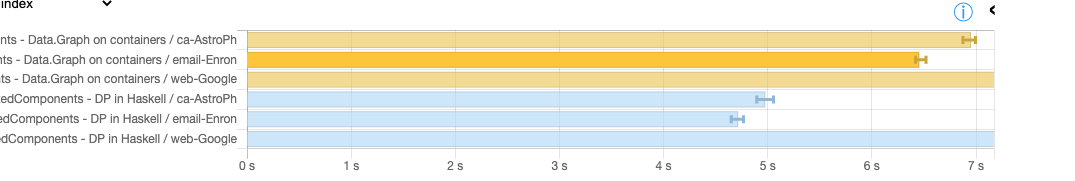
\includegraphics[width=\textwidth]{bench_1.png}
  \captionsetup{type=figure}
  \captionof{figure}{Benchmark 1 - DP in Haskell vs. Data.Graph Haskell}
  \label{fig:1}
\end{minipage}

\autoref{fig:1} shows that \acrshort{dph} solution is $1.3$ faster compare with \acrshort{hs} \texttt{containers} library. Despite this, if we zoom  in \autoref{fig:1}, it can be observed that \acrshort{dph} solution is slower compared with \acrshort{hs} \texttt{containers}; the reasons behind this have been explained in \autoref{sub:sec:e1}.
\iffalse
\begin{minipage}[t]{\linewidth}
  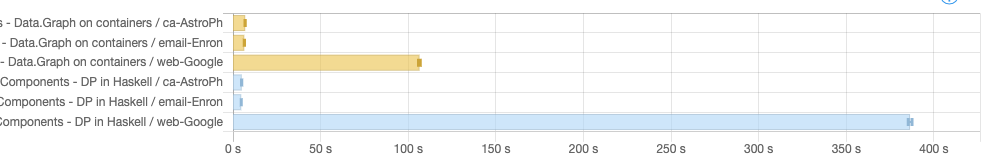
\includegraphics[width=\textwidth]{bench_2}
  \captionsetup{type=figure}
  \captionof{figure}{Benchmark 2 - DP in Haskell vs. Data.Graph Haskell}
  \label{fig:2}
\end{minipage}
\fi

 Regarding mean execution times for each implementation on each case measure by \texttt{criterion} library \cite{criterion}, we can display the following results:

\begin{table}[H]
  \centering
  \begin{tabular}{|l|l|l|l|}
   \hline
   \textbf{Network} & \textbf{\acrshort{dph}} & \textbf{\acrshort{hs} \texttt{containers}} & \textbf{Speed-up}\\
   \hline
   Enron Emails & 4.68s &  6.46s & 1.38\\
   \hline
   Astro Physics Coll Net & 4.98s & 6.95s  & 1.39\\
   \hline
   Google Web Graph & 386s & 106s & -3.64\\
   \hline
  \end{tabular}
 \caption{Mean Execution times}
 \label{table:6}
 \end{table}

These results allow for answering Question [Q2].
We already had a partial answer with the previous experiment E1 about [Q2] (\autoref{res:question}) where we have seen that the graph topology is affecting the performance and the parallelization, penalizing \acrshort{dph} for this particular case. In this benchmark, the solution against a non-parallel \texttt{containers} \mintinline{haskell}{Data.Graph} confirms the hypothesis. 

\paragraph{Diefficency Metrics}\label{sub:sub:sec:e2}
Some considerations are needed before starting to analyze the data gathered with \acrshort{dm} tool. Firstly, the tool is plotting the results according to the traces generated by the implementation, both \acrshort{dph} and \acrshort{hs} \emph{containers}. By the nature of \acrshort{dp} model, we can gather or register that timestamps as long as the model is generating results. In the case of \acrshort{hs} \texttt{containers}, this is not possible since it calculates \acrshort{wcc} at once. This is not an issue and we still can check at what point in time all \acrshort{wcc} in \acrshort{hs} \texttt{containers} are generated. In those cases, we are going to see a straight vertical line. 

It is important to remark that we needed to scale the timestamps because we have taken the time in nanoseconds. After all, the incremental generation between one \acrshort{wcc} and the other is very small but significant enough to be taken into consideration. Thus, if we left the time scale in integer milliseconds, microseconds, or nanoseconds integer part it cannot be appreciated. In case of escalation, we are discounting the nanosecond integer of the first generated results resulting in a time scale that starts close to $0$. This does not mean that the first result is generated at $0$ time, but we are discarding the previous time to focus on how the results are incrementally generated.

Having said that, we can see the results of \acrshort{dm} which are presented in two types of plots. The first one is regular line graphs in where the $x$ axis shows the time escalated when the result was generated and the $y$ axis is showing the component number that was generated at that time. The second type of plot is a radar plot in which shows how the solution is behaving on the dimensions of  \acrfull{tfft}, \acrfull{et}, \acrfull{tt}, \acrfull{comp} and \acrfull{dt} and how are the tension between them; all these metrics are higher is better. All the details about these metrics are explained here \cite{diefpaper}.

\begin{figure}[!htb]
    \centering
    \begin{minipage}{0.33\textwidth}
     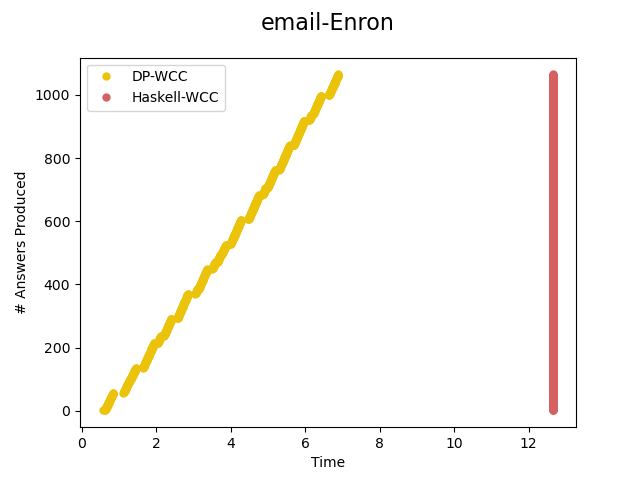
\includegraphics[width=1\linewidth, height=0.2\textheight]{email_enron}
      \caption{email-Enron \acrshort{dm}}
      \label{fig:dief:1}
    \end{minipage}%
    \begin{minipage}{0.33\textwidth}
     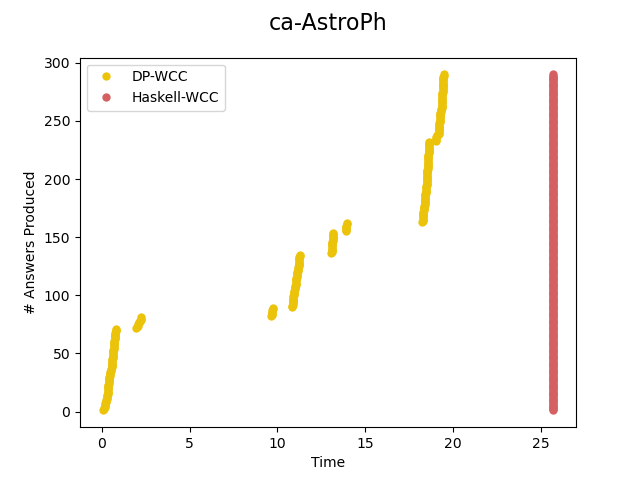
\includegraphics[width=1\linewidth, height=0.2\textheight]{ca_astroph}
      \caption{ca-AstroPh \acrshort{dm}}
      \label{fig:dief:2}
    \end{minipage}%
    \begin{minipage}{0.33\textwidth}
     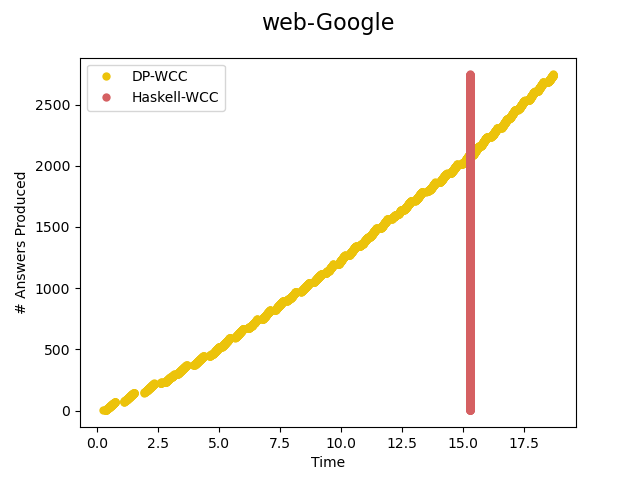
\includegraphics[width=1\linewidth, height=0.2\textheight]{web_google}
      \caption{web-Google \acrshort{dm}}
      \label{fig:dief:3}
    \end{minipage}
\end{figure}

Based on the results shown in all the figures above, all the solutions in \acrshort{dph} are being generated incrementally, but there is some difference that we would like to remark. In the case of \emph{email-Enron} and \emph{ca-AstroPh} graphs as we can see in \autoref{fig:dief:1} and \autoref{fig:dief:2}, there seems to be a more incremental generation of results. This is behavior is measured with the values of \acrfull{dt}. \emph{ca-AstroPh} as it can be seen in \autoref{fig:dief:2}, is even more incremental showing a clear separation between some results and others. The \emph{web-Google} network which is shown in \autoref{fig:dief:3}, is a little more linear and that is because all the results are being generated with very little difference in time between them. This is due to the fact of the explained reasons in \autoref{sub:sec:e1}. Having the biggest \acrshort{wcc} at the end of \emph{web-Google} \acrshort{dp} algorithm it is retaining results until the biggest \acrshort{wcc} can be solved, which takes longer. 

\begin{figure}[!htb]
    \centering
    \begin{minipage}{0.33\textwidth}
     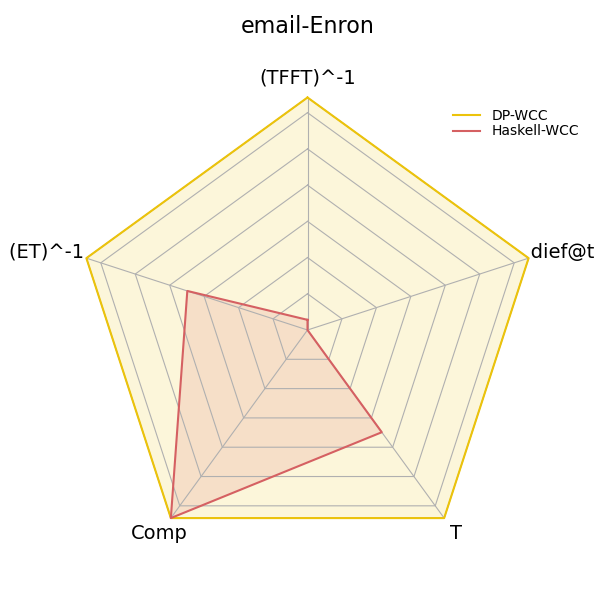
\includegraphics[width=1\linewidth, height=0.2\textheight]{email_enron_radar}
      \caption{email-Enron \acrshort{dm}}
      \label{fig:dief:rad:1}
    \end{minipage}%
    \begin{minipage}{0.33\textwidth}
     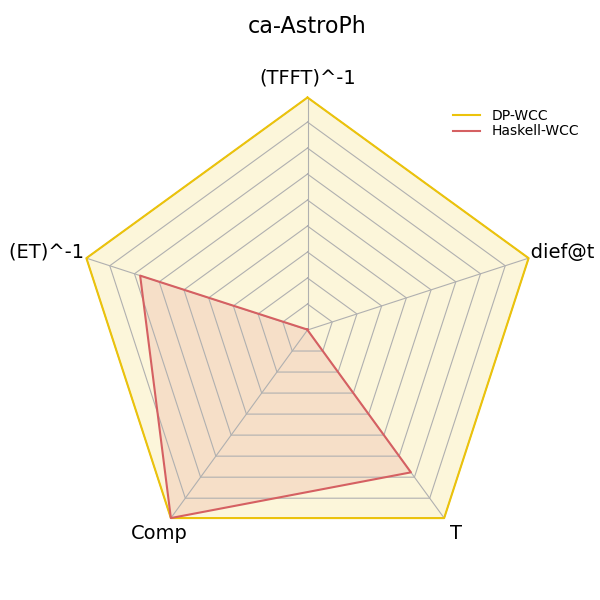
\includegraphics[width=1\linewidth, height=0.2\textheight]{ca_astroph_radar}
      \caption{ca-AstroPh \acrshort{dm}}
      \label{fig:dief:rad:2}
    \end{minipage}%
    \begin{minipage}{0.33\textwidth}
     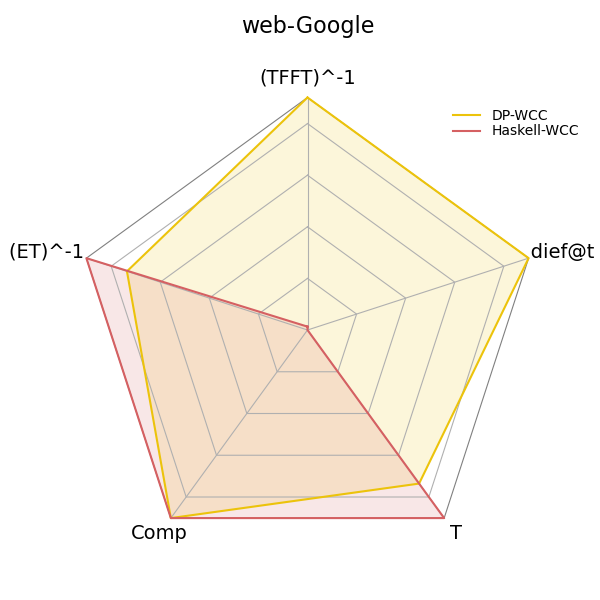
\includegraphics[width=1\linewidth, height=0.2\textheight]{web_google_radar}
      \caption{web-Google \acrshort{dm}}
      \label{fig:dief:rad:3}
    \end{minipage}
\end{figure}

As we can appreciate in the above radar plots our previous analysis can be confirmed. We can see for example that the \acrlong{tt} of \emph{web-Google} in \autoref{fig:dief:rad:3}, in the case of \acrshort{dph} is worse than \acrshort{hs} \texttt{containers}, which is not happening for the others.

In conclusion, we can say that regarding [Q2] (\autoref{res:question}) although \acrshort{dph} is faster than the traditional approach, the speed-up dimension execution factor is not always the most interest analysis that we can have, because as we have seen even when in the case of \emph{web-Google} Graph \acrshort{dph} is slower at execution, it is at least generating incremental results without the need to wait for the rest of the computations.

\subsection{Experiment: E3}
For this type of analysis, our experiment focuses on \emph{email-Enron} network \cite{netenron} only because profiling data generated by \acrshort{ghc} is big enough to conduct the analysis and on the other, and enabling profiling penalize execution time.

\paragraph{Multithreading} For analyzing parallelization and multithreading we have used \textit{ThreadScope} \cite{threadscope} which allows us to see how the parallelization is taking place on \acrshort{ghc} at a fine grained level and how the threads are distributed throughout the different cores requested with the \mintinline{bash}{-N} execution \texttt{ghc-option} flag.

\begin{minipage}[t!]{\linewidth}

  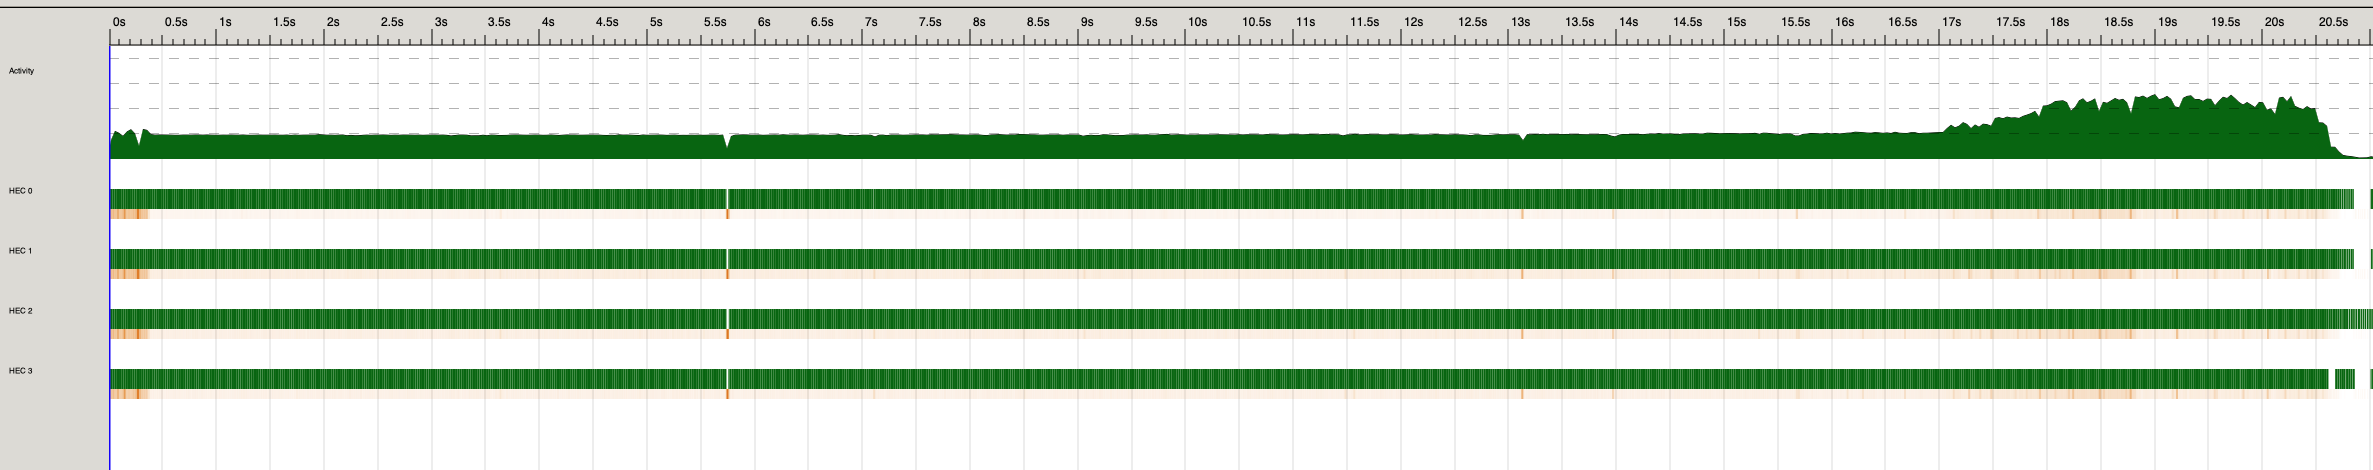
\includegraphics[width=\textwidth]{screen_1}
  \captionsetup{type=figure}
  \captionof{figure}{Threadscope Image of General Execution}
  \label{fig:3}
\end{minipage}

In \autoref{fig:3}, we can see that the parallelization is being distributed evenly among the $4$ Cores that we have set for this execution.
The distribution of the load is more intensive at the end of the execution, where \mintinline{haskell}{actor2} filter stage 
%as it can be seen in \autoref{src:haskell:3}, 
of the algorithm is taking place and different filters are reaching execution of that second actor.

Another important aspect shown in \autoref{fig:3}, is that this work is not so significant for \acrshort{ghc} and the threads and distribution of the work keeps between 1 or 2 cores during the execution time of the \mintinline{haskell}{actor1}. However, the usages increase on the second actor as pointed out before. In this regard, we can answer research questions [Q1] and [Q3] (\autoref{res:question}), verifying that \acrshort{hs} not only supports the required parallelization level but is evenly distributed across the program execution too.

Finally, it can also be appreciated that there is no sequential execution on any part of the program because the $4$ cores have \textit{CPU} activity during the whole execution time. This is because as long the program start, and because of the nature of the \acrshort{dp} model, it is spawning the \textit{Input} stage in a separated thread. This is a clear advantage for the model and the processing of the data since the program does not need to wait to do some sequential processing like reading a file, before start computing the rest of the stages.

\begin{minipage}[t!]{\linewidth}
\begin{center}
  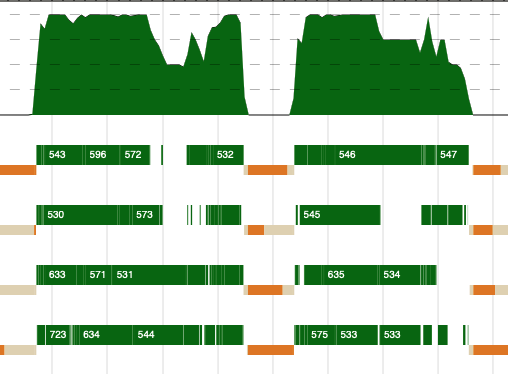
\includegraphics[width=0.6\textwidth]{screen_2}
  \captionsetup{type=figure}
  \captionof{figure}{Threadscope Image of Zoomed Fraction}
  \label{fig:4}
  \end{center}
\end{minipage}

\autoref{fig:4} zooms in on \textit{ThreadScope} output in a particular moment, approximately in the middle of the execution. We can appreciate how many threads are being spawned and by the tool and if they are evenly distributed among cores. The numbers inside green bars represent the number of threads that are being executed on that particular core (horizontal line) at that execution slot. Thus, the number of threads varies among slot execution times because as it is already known, \acrshort{ghc} implements \emph{Preemptive Scheduling} \cite{lightweightghc}.

Having said that, it can be appreciated in \autoref{fig:4} our first assumption that the load is evenly distributed because the mean number of executing threads per core is $571$.

\paragraph{Memory allocation} Another important aspect in our case is how the memory is being managed to avoid memory leaks or other non-desired behavior that increases memory allocation during the execution time. This is even more important in the particular implementation of \acrshort{wcc} using \acrshort{dp} model because it requires to maintain the set of connected components in memory throughout the execution of the program or at least until we can output the calculated \acrshort{wcc} if we reach to the last \textit{Filter} and we know that this \acrshort{wcc} cannot be enlarged anymore. 

In order to verify this, we measure memory allocation with \textit{eventlog2html} \cite{eventlog2html} which converts generated profiling memory eventlog files into graphical HTML representation. 

\begin{minipage}[t]{\linewidth}
\begin{center}
  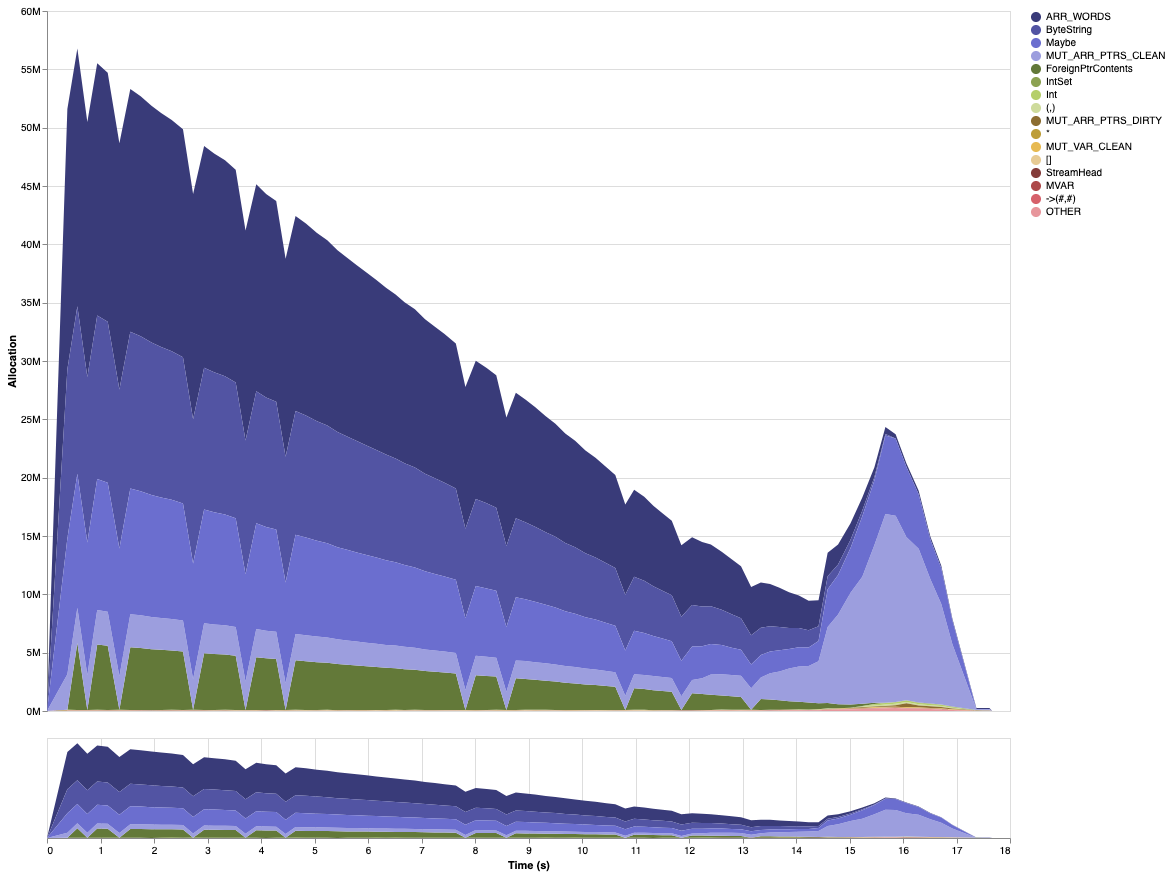
\includegraphics[width=0.6\textwidth]{visualization}
  \captionsetup{type=figure}
  \captionof{figure}{Memory Allocation}
  \label{fig:5}
  \end{center}
\end{minipage}

As we can see in \autoref{fig:5}, \acrshort{dph} does an efficient work on allocating memory since we are not using more than $57$ MB of memory during the whole execution of the program.

On the other hand, if we analyze how the memory is allocated during the execution of the program, it can also be appreciated that most of the memory is allocated at the beginning of the program and steadily decrease over time with a small peak at the end that does not overpass even half of the initial peak of $57$ MB. The explanation for this behavior is quite straightforward because at the beginning we are reading from the file and transforming a \mintinline{haskell}{ByteString} buffer to \mintinline{haskell}{(Int, Int)} edges. This is seen in the image in which the dark blue that is on top of the area is \mintinline{haskell}{ByteString} allocation. Light blue is allocation of \mintinline{haskell}{Maybe a} type which is the type that is returned by the \textit{Channels} because it can contain a value or not. Data value \mintinline{haskell}{Nothing} is indicating end of the \textit{Channel}. 
%as we can see in \autoref{src:haskell:f3}.

Another important aspect is the green area which represents \mintinline{haskell}{IntSet} allocation, which in the case of our program is the data structure that we use to gather the set of vertices that represents a \acrshort{wcc}. This means that the amount of memory used for gathering the \acrshort{wcc} itself is minimum and it is decreasing over time, which is another empirical indication that we are incrementally releasing results to the user. It can be seen as well that as long the green area reduces the lighter blue (\mintinline{haskell}{MUT_ARR_PTRS_CLEAN} \cite{ghcheap}) increases at the same time indicating that the computations for the output (releasing results) is taking place. 

Finally, according to what we have stated above, we can answer the question [Q3] (\autoref{res:question}) showing that not only memory management was efficient, but at the same time, the memory was not leaking or increasing across the running execution program.

\section{Related Work}
Several implementations for Haskell have arisen over the years to answer streaming processing models \cite{conduit, pipes, streamly}. All these libraries have their abstractions and there can do data stream processing in a fast way with their differences regarding execution time according to recent benchmarks \cite{benchstreamhs}. Although these libraries seem to be suitable for implementing \acrshort{dp} model in \acrshort{hs}, they require to know pipeline stages disposition beforehand and it is quite hard to achieve a succinct and expressive implementation of \acrshort{dp} model on such libraries. Moreover, since these libraries have been conceived with a data parallel streaming model approach instead of pipeline parallel streaming like in \acrshort{dp} model, adapting the abstraction to these tools makes it even harder to achieve.

Another kind of \acrshort{hs} implementation is described \emph{Chapter 4} subsection \emph{Pipeline Parallelism} on this book \cite{parallelbook} in the context of \mintinline{haskell}{Par} \textit{Monad}. In that work, the author describes how to encode a pipeline parallel stream model with \mintinline{haskell}{Par} \textit{Monad}. Although this could have been a proper alternative for implementing \acrshort{dph}, the parallelization level implemented at \mintinline{haskell}{Par} \textit{Monad} is achieved with sparks \cite{sparks} which is a fine grained level of parallelism inside a thread. In \acrshort{dp}, we are exploring parallelization on the pipeline stages and not data parallelization. 
\iffalse
In particular, the problem presented in \autoref{sub:sec:mot:ex} is one of the algorithms in which the amount of stages that could run in parallel is the worst case having one Stage per edge at most, but still in that scenario the number of threads can be efficiently handled by \acrshort{ghc}. Therefore, there is no need for such a fine grained parallelization level as it could be required when the data should be split into the smallest processing units as possible. 
\fi

\section{Conclusions and Ongoing Work}
We have seen that \acrlong{dp} implemented in Haskell is not only suitable but also robust. We have also seen that this implementation requires only a few lines of code, taking advantage of already built libraries and techniques as we have described in \autoref{section:prob:dp:haskell}.
We have also been able to verify that the implementation outperforms in those cases where the topology of the graph is more sparse and where the number of vertices in the largest \acrshort{wcc} is not large (all the vertices are not in one big \acrshort{wcc}). This behavior is present despite implementing a non-optimal subgraph algorithm for the specific problem of \acrshort{wcc}.
Moreover, we have measure using \acrshort{dt} metrics in \autoref{sub:sub:sec:e2}, the advantageous capability of \acrshort{dph} implementation to deliver incremental results compare with default \texttt{containers} library implementation.
Finally, we have been able to measure the principal aspects where \acrshort{dp} is strong such as pipeline parallelism and time processing showing that \acrshort{hs} can deal with the requirements for the problem without penalizing neither execution time nor memory allocation.
Another important aspect is that we still need to explore in deep the design and definition of the main DPF in \acrshort{hs} taking advantage of all the abstraction mechanisms that \acrshort{hs} provides.

In conclusion, we have gathered enough evidence to show that \acrlong{dp} is feasible in \acrlong{hs} opening a wide range of algorithms to be explored with this model, supported by a purely functional programming language.

\bibliography{Report}

\iffalse
\appendix
\section{Automated Testing and QuickCheck}\label{apx:1}
\subsection{Automated Cases}
We have defined 6 small examples with the following particularities to be automated and be tested automatically on every run of \mintinline{bash}{stack test} or \mintinline{bash}{cabal test} depends on the selected building tool. In that sense
we ensure the correctness of the principal algorithm on any possible modification and iteration. 

\begin{table}[H]
  \centering
  \begin{tabular}{|l|l|l|}
   \hline
   Graph case & Edges & Ordered (Edges)\\
   \hline
   1 \acrshort{wcc} & 5 & YES \\
   \hline
   1 \acrshort{wcc} & 5 & NO \\
   \hline
   2 \acrshort{wcc} & 8 & YES \\
   \hline
   1 \acrshort{wcc} & 6 & YES \\
   \hline
   3 \acrshort{wcc} & 11 & YES \\
   \hline
   3 \acrshort{wcc} & 11 & NO \\
   \hline
  \end{tabular}
 \caption{Test Cases}
 \label{table:apx:1}
 \end{table}

\begin{listing}[H]
\begin{minted}[fontsize=\small,numbers=left,frame=lines,framerule=2pt,framesep=2mm,baselinestretch=1.2,highlightlines={}]{haskell}      
it "Example 3 CC - Shuffle" $ do
  let input = "1 2\n 2 3\n 4 5\n 1 4\n 1 3\n 7 8\n 10 12\n 3 5\n 3 6\n 7 9\n 11 10\n"
  result <- liftIO $ runParallelWithExample input
  length result `shouldBe` 3
\end{minted}
\caption{Example \textit{hspec} Testing}
\label{src:haskell:6}
\end{listing}

\subsection{QuickCheck}
In this case, the main challenge consists of how to write \mintinline{haskell}{Arbitrary} derivations, to 
allow \textit{QuickCheck} to generate a Graph $G$ and at the same time control the number of Connected Components that we want for $G$, to verify the following property: Given a graph $G$, $cc : G \to \mathbb{N}$ is the Function that gets the Number of Connected Components of $G$.
Then,

\begin{equation}
  \forall G, cc(G) = size(DP(G))
\end{equation}

In our QuickCheck derivation this is the following:

\begin{listing}[H]
  \begin{minted}[fontsize=\small,numbers=left,frame=lines,framerule=2pt,framesep=2mm,baselinestretch=1.2,highlightlines={}]{haskell}      
newtype Edge a = Edge (a, a)
    deriving (Show, Eq, Ord)
  
newtype Graph = Graph { _gEdges :: Set (Edge Integer) } deriving (Show)
  
instance Arbitrary (Edge Integer) where
  arbitrary = do
    v1 <- getPositive <$> arbitrary
    v2 <- (getPositive <$> arbitrary) `suchThat` (/= v1)
    return $ Edge (v1, v2)
  
arbitraryGraphs :: Gen (Graph, Int)
arbitraryGraphs = do
  amount <- choose (1, 10)
  (, amount) <$> genGraph amount
  
genGraph :: Int -> Gen Graph
genGraph = fmap Graph . genConnComp
\end{minted}
\caption{QuickCheck \acrshort{dp}}
\label{src:haskell:7}
\end{listing}

We have avoided the details of \mintinline{haskell}{genConnComp} generator function, but it builds a Set of Edges 
in which the number of connected components should be the amount provided by parameter, which is randomly generated by QuickCheck.
Once we have QuickCheck generator we just need to tell QuickCheck how many examples we want to test to verify our property.

\begin{listing}[H]
\begin{minted}[fontsize=\small,numbers=left,frame=lines,framerule=2pt,framesep=2mm,baselinestretch=1.2,highlightlines={}]{haskell}      
context "Property Based Testing Examples"
  $ modifyMaxSuccess (const 1000)
  $ it "Retrieves the correct number of connected components"
  $ property
  $ forAll arbitraryGraphs 
  $ \(Graph{..}, amount) -> do 
    result <- liftIO $ runParallelWithExample $ toEdgesText _gEdges
    length result `shouldBe` amount
    
\end{minted}
\caption{QuickCheck Property Verification of \acrshort{dp}}
\label{src:haskell:8}
\end{listing}


\section{Filter}
\textbf{Filters:}\newline
In this case, the algorithm is not as succinct as the previous because here is where the 2-step calculation takes place. As explained before, each \textit{Filter} contains two sequential computations which are called \mintinline{haskell}{actor1} and \mintinline{haskell}{actor2}. The first one is responsible for gathering connected components based on the first edge from which the \textit{filter} was created.  The second \textit{actor} is responsible for \textit{combining} its calculated connected components with others that are coming from the downstream. Representing sequential computations in \acrshort{hs} is simple with \emph{Monadic} computations, which in this case \mintinline{haskell}{actor2} depends on the computation of \mintinline{haskell}{actor1}.

\begin{listing}[H]
\begin{minted}[fontsize=\small,numbers=left,frame=lines,framerule=2pt,framesep=2mm,baselinestretch=1.2,highlightlines={3,10-11,21-22}]{haskell}
newFilter :: ConnectedComponents -> ConnCompDP 
          -> DP.Channel Edge -> DP.Channel ConnectedComponents -> IO ()
newFilter conn inCh toInCh outCh = actor1 conn inCh toInCh >>= actor2 inCh toInCh outCh

actor1 :: ConnectedComponents -> ConnCompDP -> DP.Channel Edge -> IO ConnectedComponents
actor1 conn inCh toInCh = maybe finishActor doActor =<< DP.pullIn inCh
 where
  finishActor = DP.end' toInCh >> return conn

  doActor v | toConnectedComp v `intersect` conn = actor1 (toConnectedComp v <> conn) inCh toInCh
            | otherwise                          = v `DP.push'` toInCh >> actor1 conn inCh toInCh


actor2 :: ConnCompDP -> DP.Channel Edge 
       -> DP.Channel ConnectedComponents -> ConnectedComponents -> IO ()
actor2 inCh toInCh outCh conn = maybe finishActor doActor =<< DP.pullOut inCh

 where
  finishActor = conn `DP.push'` outCh >> DP.end' outCh

  doActor cc | conn `intersect` cc = actor2 inCh toInCh outCh (conn <> cc)
             | otherwise           = cc `DP.push'` outCh >> actor2 inCh toInCh outCh conn
\end{minted}
\caption{Filters \acrshort{dp} for \acrshort{wcc}}
\label{src:haskell:3}
\end{listing}

As we can see in \autoref{src:haskell:3} considering highlighted \texttt{line 21-22}, we use \mintinline{haskell}{Data.IntSet} module provided by \textbf{containers} \cite{containers} library to calculate the \textit{Intersection} and \textit{Union} of the \acrshort{wcc} calculated by this filter against  previous \acrshort{wcc} computed by other filters.\label{not:optimal}

\fi
\end{document}

